\documentclass[1p]{elsarticle_modified}
%\bibliographystyle{elsarticle-num}

%\usepackage[colorlinks]{hyperref}
%\usepackage{abbrmath_seonhwa} %\Abb, \Ascr, \Acal ,\Abf, \Afrak
\usepackage{amsfonts}
\usepackage{amssymb}
\usepackage{amsmath}
\usepackage{amsthm}
\usepackage{scalefnt}
\usepackage{amsbsy}
\usepackage{kotex}
\usepackage{caption}
\usepackage{subfig}
\usepackage{color}
\usepackage{graphicx}
\usepackage{xcolor} %% white, black, red, green, blue, cyan, magenta, yellow
\usepackage{float}
\usepackage{setspace}
\usepackage{hyperref}

\usepackage{tikz}
\usetikzlibrary{arrows}

\usepackage{multirow}
\usepackage{array} % fixed length table
\usepackage{hhline}

%%%%%%%%%%%%%%%%%%%%%
\makeatletter
\renewcommand*\env@matrix[1][\arraystretch]{%
	\edef\arraystretch{#1}%
	\hskip -\arraycolsep
	\let\@ifnextchar\new@ifnextchar
	\array{*\c@MaxMatrixCols c}}
\makeatother %https://tex.stackexchange.com/questions/14071/how-can-i-increase-the-line-spacing-in-a-matrix
%%%%%%%%%%%%%%%

\usepackage[normalem]{ulem}

\newcommand{\msout}[1]{\ifmmode\text{\sout{\ensuremath{#1}}}\else\sout{#1}\fi}
%SOURCE: \msout is \stkout macro in https://tex.stackexchange.com/questions/20609/strikeout-in-math-mode

\newcommand{\cancel}[1]{
	\ifmmode
	{\color{red}\msout{#1}}
	\else
	{\color{red}\sout{#1}}
	\fi
}

\newcommand{\add}[1]{
	{\color{blue}\uwave{#1}}
}

\newcommand{\replace}[2]{
	\ifmmode
	{\color{red}\msout{#1}}{\color{blue}\uwave{#2}}
	\else
	{\color{red}\sout{#1}}{\color{blue}\uwave{#2}}
	\fi
}

\newcommand{\Sol}{\mathcal{S}} %segment
\newcommand{\D}{D} %diagram
\newcommand{\A}{\mathcal{A}} %arc


%%%%%%%%%%%%%%%%%%%%%%%%%%%%%5 test

\def\sl{\operatorname{\textup{SL}}(2,\Cbb)}
\def\psl{\operatorname{\textup{PSL}}(2,\Cbb)}
\def\quan{\mkern 1mu \triangleright \mkern 1mu}

\theoremstyle{definition}
\newtheorem{thm}{Theorem}[section]
\newtheorem{prop}[thm]{Proposition}
\newtheorem{lem}[thm]{Lemma}
\newtheorem{ques}[thm]{Question}
\newtheorem{cor}[thm]{Corollary}
\newtheorem{defn}[thm]{Definition}
\newtheorem{exam}[thm]{Example}
\newtheorem{rmk}[thm]{Remark}
\newtheorem{alg}[thm]{Algorithm}

\newcommand{\I}{\sqrt{-1}}
\begin{document}

%\begin{frontmatter}
%
%\title{Boundary parabolic representations of knots up to 8 crossings}
%
%%% Group authors per affiliation:
%\author{Yunhi Cho} 
%\address{Department of Mathematics, University of Seoul, Seoul, Korea}
%\ead{yhcho@uos.ac.kr}
%
%
%\author{Seonhwa Kim} %\fnref{s_kim}}
%\address{Center for Geometry and Physics, Institute for Basic Science, Pohang, 37673, Korea}
%\ead{ryeona17@ibs.re.kr}
%
%\author{Hyuk Kim}
%\address{Department of Mathematical Sciences, Seoul National University, Seoul 08826, Korea}
%\ead{hyukkim@snu.ac.kr}
%
%\author{Seokbeom Yoon}
%\address{Department of Mathematical Sciences, Seoul National University, Seoul, 08826,  Korea}
%\ead{sbyoon15@snu.ac.kr}
%
%\begin{abstract}
%We find all boundary parabolic representation of knots up to 8 crossings.
%
%\end{abstract}
%\begin{keyword}
%    \MSC[2010] 57M25 
%\end{keyword}
%
%\end{frontmatter}

%\linenumbers
%\tableofcontents
%
\newcommand\colored[1]{\textcolor{white}{\rule[-0.35ex]{0.8em}{1.4ex}}\kern-0.8em\color{red} #1}%
%\newcommand\colored[1]{\textcolor{white}{ #1}\kern-2.17ex	\textcolor{white}{ #1}\kern-1.81ex	\textcolor{white}{ #1}\kern-2.15ex\color{red}#1	}

{\Large $\underline{10_{123}~(K10a_{121})}$}

\setlength{\tabcolsep}{10pt}
\renewcommand{\arraystretch}{1.6}
\vspace{1cm}\begin{tabular}{m{100pt}>{\centering\arraybackslash}m{274pt}}
\multirow{5}{120pt}{
	\centering
	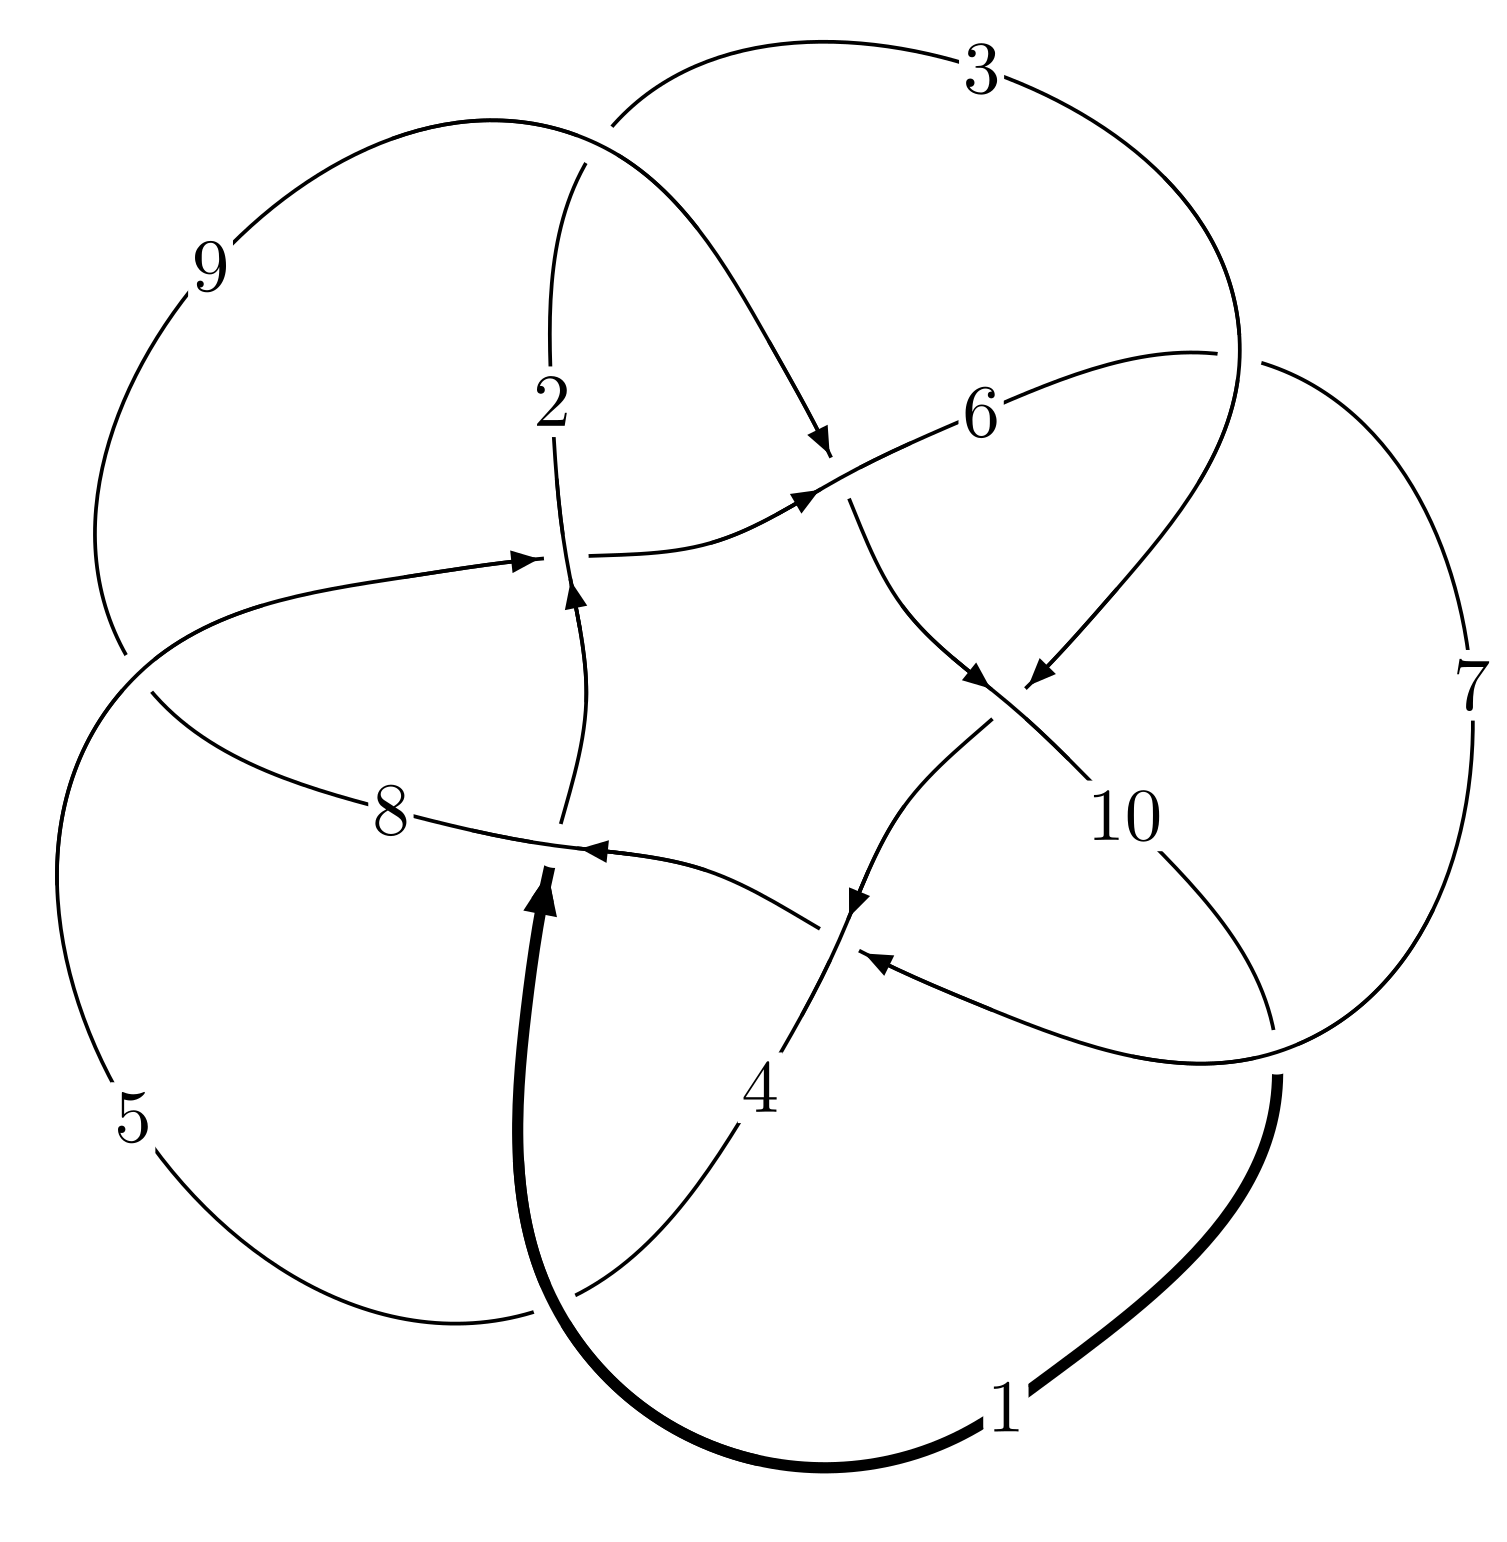
\includegraphics[width=112pt]{../../../GIT/diagram.site/Diagrams/png/207_10_123.png}\\
\ \ \ A knot diagram\footnotemark}&
\allowdisplaybreaks
\textbf{Linearized knot diagam} \\
\cline{2-2}
 &
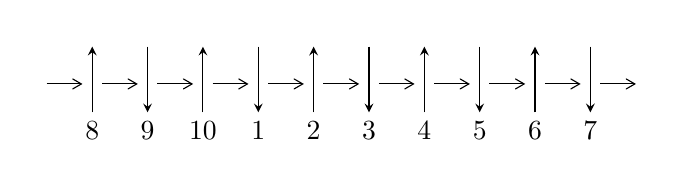
\begin{tikzpicture}[x=20pt, y=17pt]
	% nodes
	\node (C0) at (0, 0) {};
	\node (C1) at (1, 0) {};
	\node (C1U) at (1, +1) {};
	\node (C1D) at (1, -1) {8};

	\node (C2) at (2, 0) {};
	\node (C2U) at (2, +1) {};
	\node (C2D) at (2, -1) {9};

	\node (C3) at (3, 0) {};
	\node (C3U) at (3, +1) {};
	\node (C3D) at (3, -1) {10};

	\node (C4) at (4, 0) {};
	\node (C4U) at (4, +1) {};
	\node (C4D) at (4, -1) {1};

	\node (C5) at (5, 0) {};
	\node (C5U) at (5, +1) {};
	\node (C5D) at (5, -1) {2};

	\node (C6) at (6, 0) {};
	\node (C6U) at (6, +1) {};
	\node (C6D) at (6, -1) {3};

	\node (C7) at (7, 0) {};
	\node (C7U) at (7, +1) {};
	\node (C7D) at (7, -1) {4};

	\node (C8) at (8, 0) {};
	\node (C8U) at (8, +1) {};
	\node (C8D) at (8, -1) {5};

	\node (C9) at (9, 0) {};
	\node (C9U) at (9, +1) {};
	\node (C9D) at (9, -1) {6};

	\node (C10) at (10, 0) {};
	\node (C10U) at (10, +1) {};
	\node (C10D) at (10, -1) {7};
	\node (C11) at (11, 0) {};

	% arrows
	\draw[->,>={angle 60}]
	(C0) edge (C1) (C1) edge (C2) (C2) edge (C3) (C3) edge (C4) (C4) edge (C5) (C5) edge (C6) (C6) edge (C7) (C7) edge (C8) (C8) edge (C9) (C9) edge (C10) (C10) edge (C11) ;	\draw[->,>=stealth]
	(C1D) edge (C1U) (C2U) edge (C2D) (C3D) edge (C3U) (C4U) edge (C4D) (C5D) edge (C5U) (C6U) edge (C6D) (C7D) edge (C7U) (C8U) edge (C8D) (C9D) edge (C9U) (C10U) edge (C10D) ;
	\end{tikzpicture} \\
\hhline{~~} \\& 
\textbf{Solving Sequence} \\ \cline{2-2} 
 &
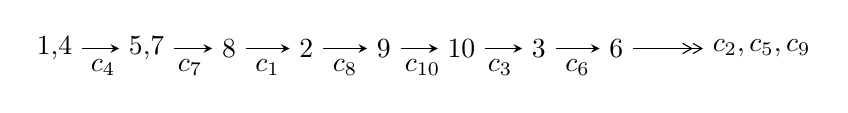
\begin{tikzpicture}[x=28pt, y=7pt]
	% node
	\node (A0) at (-1/8, 0) {1,4};
	\node (A1) at (17/16, 0) {5,7};
	\node (A2) at (17/8, 0) {8};
	\node (A3) at (25/8, 0) {2};
	\node (A4) at (33/8, 0) {9};
	\node (A5) at (41/8, 0) {10};
	\node (A6) at (49/8, 0) {3};
	\node (A7) at (57/8, 0) {6};
	\node (C1) at (1/2, -1) {$c_{4}$};
	\node (C2) at (13/8, -1) {$c_{7}$};
	\node (C3) at (21/8, -1) {$c_{1}$};
	\node (C4) at (29/8, -1) {$c_{8}$};
	\node (C5) at (37/8, -1) {$c_{10}$};
	\node (C6) at (45/8, -1) {$c_{3}$};
	\node (C7) at (53/8, -1) {$c_{6}$};
	\node (A8) at (9, 0) {$c_{2},c_{5},c_{9}$};

	% edge
	\draw[->,>=stealth]	
	(A0) edge (A1) (A1) edge (A2) (A2) edge (A3) (A3) edge (A4) (A4) edge (A5) (A5) edge (A6) (A6) edge (A7) ;
	\draw[->>,>={angle 60}]	
	(A7) edge (A8);
\end{tikzpicture} \\ 

\end{tabular} \\

\footnotetext{
The image of knot diagram is generated by the software ``\textbf{Draw programme}" developed by Andrew Bartholomew(\url{http://www.layer8.co.uk/maths/draw/index.htm\#Running-draw}), where we modified some parts for our purpose(\url{https://github.com/CATsTAILs/LinksPainter}).
}\phantom \\ \newline 
\centering \textbf{Ideals for irreducible components\footnotemark of $X_{\text{par}}$} 
 
\begin{align*}
I^u_{1}&=\langle 
u^3+2 u^2+b+2 u+1,\;a-1,\;u^4+3 u^3+4 u^2+2 u+1\rangle \\
I^u_{2}&=\langle 
u^3+b+1,\;a+1,\;u^4- u^3+2 u-1\rangle \\
I^u_{3}&=\langle 
-6 u^9+3 u^8+17 u^7-22 u^6-19 u^5+31 u^4+5 u^3-22 u^2+2 b+2 u+6,\\
\phantom{I^u_{3}}&\phantom{= \langle  }6 u^9-21 u^8+13 u^7+31 u^6-48 u^5-5 u^4+36 u^3-13 u^2+2 a-9 u+2,\\
\phantom{I^u_{3}}&\phantom{= \langle  }3 u^{10}-6 u^9- u^8+14 u^7-8 u^6-10 u^5+11 u^4+2 u^3-5 u^2+1\rangle \\
I^u_{4}&=\langle 
18 u^9-30 u^8-9 u^7+67 u^6-26 u^5-41 u^4+35 u^3+7 u^2+2 b-8 u,\;a-1,\\
\phantom{I^u_{4}}&\phantom{= \langle  }3 u^{10}-6 u^9- u^8+14 u^7-8 u^6-10 u^5+11 u^4+2 u^3-5 u^2+1\rangle \\
I^u_{5}&=\langle 
-2 u^9+7 u^8-14 u^7+19 u^6-27 u^5+34 u^4-40 u^3+33 u^2+2 b-22 u+6,\\
\phantom{I^u_{5}}&\phantom{= \langle  }-4 u^9+14 u^8-28 u^7+41 u^6-58 u^5+73 u^4-81 u^3+76 u^2+6 a-50 u+23,\\
\phantom{I^u_{5}}&\phantom{= \langle  }u^{10}-4 u^9+9 u^8-14 u^7+20 u^6-26 u^5+31 u^4-30 u^3+23 u^2-12 u+3\rangle \\
I^u_{6}&=\langle 
5 u^9-20 u^8+42 u^7-61 u^6+85 u^5-109 u^4+125 u^3-114 u^2+6 b+79 u-30,\\
\phantom{I^u_{6}}&\phantom{= \langle  }u^9+2 u^8-9 u^7+19 u^6-22 u^5+34 u^4-41 u^3+54 u^2+6 a-40 u+24,\\
\phantom{I^u_{6}}&\phantom{= \langle  }u^{10}-4 u^9+9 u^8-14 u^7+20 u^6-26 u^5+31 u^4-30 u^3+23 u^2-12 u+3\rangle \\
I^u_{7}&=\langle 
-17 u^9-123 u^8-488 u^7-1301 u^6-2539 u^5-3687 u^4-4024 u^3-3128 u^2+144 b-1616 u-496,\\
\phantom{I^u_{7}}&\phantom{= \langle  }u^9+21 u^8+118 u^7+397 u^6+917 u^5+1557 u^4+1958 u^3+1792 u^2+96 a+1096 u+416,\\
\phantom{I^u_{7}}&\phantom{= \langle  }u^{10}+7 u^9+28 u^8+77 u^7+159 u^6+251 u^5+308 u^4+288 u^3+200 u^2+96 u+32\rangle \\
I^u_{8}&=\langle 
a^3 u^2-2 a^2 u^2+a^2 u+u^2 a+b a+a^2- a u- a+1,\;a^2 u^2- u^2 a+b u+a u+b+a,\;u^3 a^2- u^3 a+a u- u-1\rangle \\
\\
\end{align*}
\raggedright * 7 irreducible components of $\dim_{\mathbb{C}}=0$, with total 58 representations.\\
\raggedright * 1 irreducible components of $\dim_{\mathbb{C}}=1$ \\
\footnotetext{All coefficients of polynomials are rational numbers. But the coefficients are sometimes approximated in decimal forms when there is not enough margin.}
\newpage
\renewcommand{\arraystretch}{1}
\centering \section*{I. $I^u_{1}= \langle u^3+2 u^2+b+2 u+1,\;a-1,\;u^4+3 u^3+4 u^2+2 u+1 \rangle$}
\flushleft \textbf{(i) Arc colorings}\\
\begin{tabular}{m{7pt} m{180pt} m{7pt} m{180pt} }
\flushright $a_{1}=$&$\begin{pmatrix}0\\u\end{pmatrix}$ \\
\flushright $a_{4}=$&$\begin{pmatrix}1\\0\end{pmatrix}$ \\
\flushright $a_{5}=$&$\begin{pmatrix}1\\u^2\end{pmatrix}$ \\
\flushright $a_{7}=$&$\begin{pmatrix}1\\- u^3-2 u^2-2 u-1\end{pmatrix}$ \\
\flushright $a_{8}=$&$\begin{pmatrix}- u^3-2 u^2-2 u\\- u^3-2 u^2-2 u-1\end{pmatrix}$ \\
\flushright $a_{2}=$&$\begin{pmatrix}u^2+u+1\\- u^3- u^2\end{pmatrix}$ \\
\flushright $a_{9}=$&$\begin{pmatrix}- u^3-2 u^2- u\\-2 u^2-2 u-1\end{pmatrix}$ \\
\flushright $a_{10}=$&$\begin{pmatrix}u\\u^3+2 u^2+2 u+1\end{pmatrix}$ \\
\flushright $a_{3}=$&$\begin{pmatrix}- u^3-2 u^2- u\\u^3+u^2+u\end{pmatrix}$ \\
\flushright $a_{6}=$&$\begin{pmatrix}- u^3-3 u^2-2 u\\u^3+u^2\end{pmatrix}$\\&\end{tabular}
\flushleft \textbf{(ii) Obstruction class $= -1$}\\~\\
\flushleft \textbf{(iii) Cusp Shapes $= -5 u^3-10 u^2-15 u-5$}\\~\\
\newpage\renewcommand{\arraystretch}{1}
\flushleft \textbf{(iv) u-Polynomials at the component}\newline \\
\begin{tabular}{m{50pt}|m{274pt}}
Crossings & \hspace{64pt}u-Polynomials at each crossing \\
\hline $$\begin{aligned}c_{1},c_{3},c_{5}\\c_{7},c_{9}\end{aligned}$$&$\begin{aligned}
&u^4-3 u^3+4 u^2-2 u+1
\end{aligned}$\\
\hline $$\begin{aligned}c_{2},c_{4},c_{6}\\c_{8},c_{10}\end{aligned}$$&$\begin{aligned}
&u^4+3 u^3+4 u^2+2 u+1
\end{aligned}$\\
\hline
\end{tabular}\\~\\
\newpage\renewcommand{\arraystretch}{1}
\flushleft \textbf{(v) Riley Polynomials at the component}\newline \\
\begin{tabular}{m{50pt}|m{274pt}}
Crossings & \hspace{64pt}Riley Polynomials at each crossing \\
\hline $$\begin{aligned}c_{1},c_{2},c_{3}\\c_{4},c_{5},c_{6}\\c_{7},c_{8},c_{9}\\c_{10}\end{aligned}$$&$\begin{aligned}
&y^4- y^3+6 y^2+4 y+1
\end{aligned}$\\
\hline
\end{tabular}\\~\\
\newpage\flushleft \textbf{(vi) Complex Volumes and Cusp Shapes}
$$\begin{array}{c|c|c}  
\text{Solutions to }I^u_{1}& \I (\text{vol} + \sqrt{-1}CS) & \text{Cusp shape}\\
 \hline 
\begin{aligned}
u &= -0.190983 + 0.587785 I \\
a &= \phantom{-}1.00000\phantom{ +0.000000I} \\
b &= -0.190983 - 0.587785 I\end{aligned}
 & \phantom{-0.000000 -}1.38939 I & \phantom{-0.000000 } 0. - 5.87785 I \\ \hline\begin{aligned}
u &= -0.190983 - 0.587785 I \\
a &= \phantom{-}1.00000\phantom{ +0.000000I} \\
b &= -0.190983 + 0.587785 I\end{aligned}
 & \phantom{-0.000000 } -1.38939 I & \phantom{-0.000000 -}0. + 5.87785 I \\ \hline\begin{aligned}
u &= -1.30902 + 0.95106 I \\
a &= \phantom{-}1.00000\phantom{ +0.000000I} \\
b &= -1.30902 - 0.95106 I\end{aligned}
 & \phantom{-0.000000 -}17.0857 I & \phantom{-0.000000 } 0. - 9.51057 I \\ \hline\begin{aligned}
u &= -1.30902 - 0.95106 I \\
a &= \phantom{-}1.00000\phantom{ +0.000000I} \\
b &= -1.30902 + 0.95106 I\end{aligned}
 & \phantom{-0.000000 } -17.0857 I & \phantom{-0.000000 -}0. + 9.51057 I\\
 \hline 
 \end{array}$$\newpage\newpage\renewcommand{\arraystretch}{1}
\centering \section*{II. $I^u_{2}= \langle u^3+b+1,\;a+1,\;u^4- u^3+2 u-1 \rangle$}
\flushleft \textbf{(i) Arc colorings}\\
\begin{tabular}{m{7pt} m{180pt} m{7pt} m{180pt} }
\flushright $a_{1}=$&$\begin{pmatrix}0\\u\end{pmatrix}$ \\
\flushright $a_{4}=$&$\begin{pmatrix}1\\0\end{pmatrix}$ \\
\flushright $a_{5}=$&$\begin{pmatrix}1\\u^2\end{pmatrix}$ \\
\flushright $a_{7}=$&$\begin{pmatrix}-1\\- u^3-1\end{pmatrix}$ \\
\flushright $a_{8}=$&$\begin{pmatrix}- u^3-2\\- u^3-1\end{pmatrix}$ \\
\flushright $a_{2}=$&$\begin{pmatrix}2 u^3- u^2- u+3\\u^3- u^2+2\end{pmatrix}$ \\
\flushright $a_{9}=$&$\begin{pmatrix}- u^3+u-2\\-1\end{pmatrix}$ \\
\flushright $a_{10}=$&$\begin{pmatrix}u\\u^3+1\end{pmatrix}$ \\
\flushright $a_{3}=$&$\begin{pmatrix}u^3- u+2\\u^3- u^2- u+2\end{pmatrix}$ \\
\flushright $a_{6}=$&$\begin{pmatrix}- u^3+u^2-2\\- u^3+u^2-2\end{pmatrix}$\\&\end{tabular}
\flushleft \textbf{(ii) Obstruction class $= 1$}\\~\\
\flushleft \textbf{(iii) Cusp Shapes $= 5 u^3+5 u+5$}\\~\\
\newpage\renewcommand{\arraystretch}{1}
\flushleft \textbf{(iv) u-Polynomials at the component}\newline \\
\begin{tabular}{m{50pt}|m{274pt}}
Crossings & \hspace{64pt}u-Polynomials at each crossing \\
\hline $$\begin{aligned}c_{1},c_{3},c_{5}\\c_{7},c_{9}\end{aligned}$$&$\begin{aligned}
&u^4+u^3-2 u-1
\end{aligned}$\\
\hline $$\begin{aligned}c_{2},c_{4},c_{6}\\c_{8},c_{10}\end{aligned}$$&$\begin{aligned}
&u^4- u^3+2 u-1
\end{aligned}$\\
\hline
\end{tabular}\\~\\
\newpage\renewcommand{\arraystretch}{1}
\flushleft \textbf{(v) Riley Polynomials at the component}\newline \\
\begin{tabular}{m{50pt}|m{274pt}}
Crossings & \hspace{64pt}Riley Polynomials at each crossing \\
\hline $$\begin{aligned}c_{1},c_{2},c_{3}\\c_{4},c_{5},c_{6}\\c_{7},c_{8},c_{9}\\c_{10}\end{aligned}$$&$\begin{aligned}
&y^4- y^3+2 y^2-4 y+1
\end{aligned}$\\
\hline
\end{tabular}\\~\\
\newpage\flushleft \textbf{(vi) Complex Volumes and Cusp Shapes}
$$\begin{array}{c|c|c}  
\text{Solutions to }I^u_{2}& \I (\text{vol} + \sqrt{-1}CS) & \text{Cusp shape}\\
 \hline 
\begin{aligned}
u &= -1.15372\phantom{ +0.000000I} \\
a &= -1.00000\phantom{ +0.000000I} \\
b &= \phantom{-}0.535687\phantom{ +0.000000I}\end{aligned}
 & -4.48216\phantom{ +0.000000I} & -8.44700\phantom{ +0.000000I} \\ \hline\begin{aligned}
u &= \phantom{-}0.809017 + 0.981593 I \\
a &= -1.00000\phantom{ +0.000000I} \\
b &= \phantom{-}0.809017 - 0.981593 I\end{aligned}
 & \phantom{-0.000000 } -9.37207 I & \phantom{-0.000000 -}0. + 9.81593 I \\ \hline\begin{aligned}
u &= \phantom{-}0.809017 - 0.981593 I \\
a &= -1.00000\phantom{ +0.000000I} \\
b &= \phantom{-}0.809017 + 0.981593 I\end{aligned}
 & \phantom{-0.000000 -}9.37207 I & \phantom{-0.000000 } 0. - 9.81593 I \\ \hline\begin{aligned}
u &= \phantom{-}0.535687\phantom{ +0.000000I} \\
a &= -1.00000\phantom{ +0.000000I} \\
b &= -1.15372\phantom{ +0.000000I}\end{aligned}
 & \phantom{-}4.48216\phantom{ +0.000000I} & \phantom{-}8.44700\phantom{ +0.000000I}\\
 \hline 
 \end{array}$$\newpage\newpage\renewcommand{\arraystretch}{1}
\centering \section*{III. $I^u_{3}= \langle -6 u^9+3 u^8+\cdots+2 b+6,\;6 u^9-21 u^8+\cdots+2 a+2,\;3 u^{10}-6 u^9+\cdots-5 u^2+1 \rangle$}
\flushleft \textbf{(i) Arc colorings}\\
\begin{tabular}{m{7pt} m{180pt} m{7pt} m{180pt} }
\flushright $a_{1}=$&$\begin{pmatrix}0\\u\end{pmatrix}$ \\
\flushright $a_{4}=$&$\begin{pmatrix}1\\0\end{pmatrix}$ \\
\flushright $a_{5}=$&$\begin{pmatrix}1\\u^2\end{pmatrix}$ \\
\flushright $a_{7}=$&$\begin{pmatrix}-3 u^9+\frac{21}{2} u^8+\cdots+\frac{9}{2} u-1\\3 u^9-\frac{3}{2} u^8+\cdots- u-3\end{pmatrix}$ \\
\flushright $a_{8}=$&$\begin{pmatrix}9 u^8-15 u^7+\cdots+\frac{7}{2} u-4\\3 u^9-\frac{3}{2} u^8+\cdots- u-3\end{pmatrix}$ \\
\flushright $a_{2}=$&$\begin{pmatrix}12 u^9-\frac{27}{2} u^8+\cdots-11 u-3\\\frac{3}{2} u^9-3 u^8+\cdots-3 u-\frac{1}{2}\end{pmatrix}$ \\
\flushright $a_{9}=$&$\begin{pmatrix}9 u^8-15 u^7+\cdots+\frac{9}{2} u-4\\3 u^9-\frac{3}{2} u^8+\cdots- u-3\end{pmatrix}$ \\
\flushright $a_{10}=$&$\begin{pmatrix}6 u^9-\frac{9}{2} u^8+\cdots-\frac{5}{2} u-\frac{1}{2}\\\frac{9}{2} u^9-6 u^8+\cdots-\frac{7}{2} u-2\end{pmatrix}$ \\
\flushright $a_{3}=$&$\begin{pmatrix}-3 u^8+3 u^7+4 u^6-10 u^5-2 u^4+8 u^3-3 u^2-5 u+1\\-\frac{9}{2} u^9+\frac{9}{2} u^8+\cdots+2 u+\frac{5}{2}\end{pmatrix}$ \\
\flushright $a_{6}=$&$\begin{pmatrix}-21 u^9+\frac{75}{2} u^8+\cdots+\frac{21}{2} u+\frac{1}{2}\\-6 u^9+\frac{21}{2} u^8+\cdots+\frac{9}{2} u+1\end{pmatrix}$\\&\end{tabular}
\flushleft \textbf{(ii) Obstruction class $= -1$}\\~\\
\flushleft \textbf{(iii) Cusp Shapes $= 12 u^9+6 u^8-64 u^7+52 u^6+90 u^5-110 u^4-30 u^3+86 u^2-4 u-24$}\\~\\
\newpage\renewcommand{\arraystretch}{1}
\flushleft \textbf{(iv) u-Polynomials at the component}\newline \\
\begin{tabular}{m{50pt}|m{274pt}}
Crossings & \hspace{64pt}u-Polynomials at each crossing \\
\hline $$\begin{aligned}c_{1}\end{aligned}$$&$\begin{aligned}
&u^{10}-7 u^9+\cdots-96 u+32
\end{aligned}$\\
\hline $$\begin{aligned}c_{2},c_{10}\end{aligned}$$&$\begin{aligned}
&u^{10}-4 u^9+\cdots-12 u+3
\end{aligned}$\\
\hline $$\begin{aligned}c_{3},c_{9}\end{aligned}$$&$\begin{aligned}
&3(3 u^{10}+6 u^9- u^8-14 u^7-8 u^6+10 u^5+11 u^4-2 u^3-5 u^2+1)
\end{aligned}$\\
\hline $$\begin{aligned}c_{4},c_{8}\end{aligned}$$&$\begin{aligned}
&3(3 u^{10}-6 u^9- u^8+14 u^7-8 u^6-10 u^5+11 u^4+2 u^3-5 u^2+1)
\end{aligned}$\\
\hline $$\begin{aligned}c_{5},c_{7}\end{aligned}$$&$\begin{aligned}
&u^{10}+4 u^9+\cdots+12 u+3
\end{aligned}$\\
\hline $$\begin{aligned}c_{6}\end{aligned}$$&$\begin{aligned}
&u^{10}+7 u^9+\cdots+96 u+32
\end{aligned}$\\
\hline
\end{tabular}\\~\\
\newpage\renewcommand{\arraystretch}{1}
\flushleft \textbf{(v) Riley Polynomials at the component}\newline \\
\begin{tabular}{m{50pt}|m{274pt}}
Crossings & \hspace{64pt}Riley Polynomials at each crossing \\
\hline $$\begin{aligned}c_{1},c_{6}\end{aligned}$$&$\begin{aligned}
&y^{10}+7 y^9+\cdots+3584 y+1024
\end{aligned}$\\
\hline $$\begin{aligned}c_{2},c_{5},c_{7}\\c_{10}\end{aligned}$$&$\begin{aligned}
&y^{10}+2 y^9+9 y^8+18 y^7+36 y^6+48 y^5+39 y^4+22 y^3-5 y^2-6 y+9
\end{aligned}$\\
\hline $$\begin{aligned}c_{3},c_{4},c_{8}\\c_{9}\end{aligned}$$&$\begin{aligned}
&9(9 y^{10}-42 y^9+\cdots-10 y+1)
\end{aligned}$\\
\hline
\end{tabular}\\~\\
\newpage\flushleft \textbf{(vi) Complex Volumes and Cusp Shapes}
$$\begin{array}{c|c|c}  
\text{Solutions to }I^u_{3}& \I (\text{vol} + \sqrt{-1}CS) & \text{Cusp shape}\\
 \hline 
\begin{aligned}
u &= -0.983280 + 0.164908 I \\
a &= -0.716079 + 0.118069 I \\
b &= \phantom{-}0.724687 - 0.940396 I\end{aligned}
 & -3.61397 + 2.21654 I & -5.38699 - 4.72022 I \\ \hline\begin{aligned}
u &= -0.983280 - 0.164908 I \\
a &= -0.716079 - 0.118069 I \\
b &= \phantom{-}0.724687 + 0.940396 I\end{aligned}
 & -3.61397 - 2.21654 I & -5.38699 + 4.72022 I \\ \hline\begin{aligned}
u &= \phantom{-}0.707358 + 0.648629 I \\
a &= -0.105697 - 1.232530 I \\
b &= \phantom{-}0.684636 - 0.234182 I\end{aligned}
 & \phantom{-}3.61397 - 2.21654 I & \phantom{-}5.38699 + 4.72022 I \\ \hline\begin{aligned}
u &= \phantom{-}0.707358 - 0.648629 I \\
a &= -0.105697 + 1.232530 I \\
b &= \phantom{-}0.684636 + 0.234182 I\end{aligned}
 & \phantom{-}3.61397 + 2.21654 I & \phantom{-}5.38699 - 4.72022 I \\ \hline\begin{aligned}
u &= \phantom{-}0.744942 + 0.201707 I \\
a &= \phantom{-}1.81391 + 0.74172 I \\
b &= -0.719811 + 1.046890 I\end{aligned}
 & -2.49243 - 8.64801 I & -4.04126 + 7.50135 I \\ \hline\begin{aligned}
u &= \phantom{-}0.744942 - 0.201707 I \\
a &= \phantom{-}1.81391 - 0.74172 I \\
b &= -0.719811 - 1.046890 I\end{aligned}
 & -2.49243 + 8.64801 I & -4.04126 - 7.50135 I \\ \hline\begin{aligned}
u &= \phantom{-}1.081500 + 0.798609 I \\
a &= -0.893282 - 0.308372 I \\
b &= \phantom{-}1.20165 - 0.91842 I\end{aligned}
 & \phantom{-}2.49243 - 8.64801 I & \phantom{-}4.04126 + 7.50135 I \\ \hline\begin{aligned}
u &= \phantom{-}1.081500 - 0.798609 I \\
a &= -0.893282 + 0.308372 I \\
b &= \phantom{-}1.20165 + 0.91842 I\end{aligned}
 & \phantom{-}2.49243 + 8.64801 I & \phantom{-}4.04126 - 7.50135 I \\ \hline\begin{aligned}
u &= -0.550514 + 0.187402 I \\
a &= \phantom{-}0.40115 - 1.75920 I \\
b &= \phantom{-}0.108840 - 1.043640 I\end{aligned}
 & \phantom{-0.000000 -}0.806279 I & \phantom{-0.000000 } 0. - 8.22652 I \\ \hline\begin{aligned}
u &= -0.550514 - 0.187402 I \\
a &= \phantom{-}0.40115 + 1.75920 I \\
b &= \phantom{-}0.108840 + 1.043640 I\end{aligned}
 & \phantom{-0.000000 } -0.806279 I & \phantom{-0.000000 -}0. + 8.22652 I\\
 \hline 
 \end{array}$$\newpage\newpage\renewcommand{\arraystretch}{1}
\centering \section*{IV. $I^u_{4}= \langle 18 u^9-30 u^8+\cdots+2 b-8 u,\;a-1,\;3 u^{10}-6 u^9+\cdots-5 u^2+1 \rangle$}
\flushleft \textbf{(i) Arc colorings}\\
\begin{tabular}{m{7pt} m{180pt} m{7pt} m{180pt} }
\flushright $a_{1}=$&$\begin{pmatrix}0\\u\end{pmatrix}$ \\
\flushright $a_{4}=$&$\begin{pmatrix}1\\0\end{pmatrix}$ \\
\flushright $a_{5}=$&$\begin{pmatrix}1\\u^2\end{pmatrix}$ \\
\flushright $a_{7}=$&$\begin{pmatrix}1\\-9 u^9+15 u^8+\cdots-\frac{7}{2} u^2+4 u\end{pmatrix}$ \\
\flushright $a_{8}=$&$\begin{pmatrix}-9 u^9+15 u^8+\cdots+4 u+1\\-9 u^9+15 u^8+\cdots-\frac{7}{2} u^2+4 u\end{pmatrix}$ \\
\flushright $a_{2}=$&$\begin{pmatrix}-\frac{3}{2} u^9-\frac{3}{2} u^8+\cdots-3 u+\frac{5}{2}\\\frac{3}{2} u^9-3 u^8+\cdots-3 u-\frac{1}{2}\end{pmatrix}$ \\
\flushright $a_{9}=$&$\begin{pmatrix}-\frac{9}{2} u^9+\frac{15}{2} u^8+\cdots+3 u+2\\-6 u^9+\frac{21}{2} u^8+\cdots+\frac{5}{2} u-\frac{1}{2}\end{pmatrix}$ \\
\flushright $a_{10}=$&$\begin{pmatrix}u\\-3 u^9+\frac{3}{2} u^8+\cdots+u+3\end{pmatrix}$ \\
\flushright $a_{3}=$&$\begin{pmatrix}-\frac{9}{2} u^9+\frac{15}{2} u^8+\cdots+3 u+2\\-\frac{9}{2} u^9+6 u^8+\cdots+\frac{5}{2} u+\frac{1}{2}\end{pmatrix}$ \\
\flushright $a_{6}=$&$\begin{pmatrix}-\frac{3}{2} u^9+\frac{3}{2} u^8+\cdots- u-\frac{3}{2}\\\frac{3}{2} u^9-\frac{3}{2} u^8+\cdots-\frac{3}{2} u-2\end{pmatrix}$\\&\end{tabular}
\flushleft \textbf{(ii) Obstruction class $= -1$}\\~\\
\flushleft \textbf{(iii) Cusp Shapes $= 12 u^9+6 u^8-64 u^7+52 u^6+90 u^5-110 u^4-30 u^3+86 u^2-4 u-24$}\\~\\
\newpage\renewcommand{\arraystretch}{1}
\flushleft \textbf{(iv) u-Polynomials at the component}\newline \\
\begin{tabular}{m{50pt}|m{274pt}}
Crossings & \hspace{64pt}u-Polynomials at each crossing \\
\hline $$\begin{aligned}c_{1},c_{3}\end{aligned}$$&$\begin{aligned}
&u^{10}+4 u^9+\cdots+12 u+3
\end{aligned}$\\
\hline $$\begin{aligned}c_{2}\end{aligned}$$&$\begin{aligned}
&u^{10}+7 u^9+\cdots+96 u+32
\end{aligned}$\\
\hline $$\begin{aligned}c_{4},c_{10}\end{aligned}$$&$\begin{aligned}
&3(3 u^{10}-6 u^9- u^8+14 u^7-8 u^6-10 u^5+11 u^4+2 u^3-5 u^2+1)
\end{aligned}$\\
\hline $$\begin{aligned}c_{5},c_{9}\end{aligned}$$&$\begin{aligned}
&3(3 u^{10}+6 u^9- u^8-14 u^7-8 u^6+10 u^5+11 u^4-2 u^3-5 u^2+1)
\end{aligned}$\\
\hline $$\begin{aligned}c_{6},c_{8}\end{aligned}$$&$\begin{aligned}
&u^{10}-4 u^9+\cdots-12 u+3
\end{aligned}$\\
\hline $$\begin{aligned}c_{7}\end{aligned}$$&$\begin{aligned}
&u^{10}-7 u^9+\cdots-96 u+32
\end{aligned}$\\
\hline
\end{tabular}\\~\\
\newpage\renewcommand{\arraystretch}{1}
\flushleft \textbf{(v) Riley Polynomials at the component}\newline \\
\begin{tabular}{m{50pt}|m{274pt}}
Crossings & \hspace{64pt}Riley Polynomials at each crossing \\
\hline $$\begin{aligned}c_{1},c_{3},c_{6}\\c_{8}\end{aligned}$$&$\begin{aligned}
&y^{10}+2 y^9+9 y^8+18 y^7+36 y^6+48 y^5+39 y^4+22 y^3-5 y^2-6 y+9
\end{aligned}$\\
\hline $$\begin{aligned}c_{2},c_{7}\end{aligned}$$&$\begin{aligned}
&y^{10}+7 y^9+\cdots+3584 y+1024
\end{aligned}$\\
\hline $$\begin{aligned}c_{4},c_{5},c_{9}\\c_{10}\end{aligned}$$&$\begin{aligned}
&9(9 y^{10}-42 y^9+\cdots-10 y+1)
\end{aligned}$\\
\hline
\end{tabular}\\~\\
\newpage\flushleft \textbf{(vi) Complex Volumes and Cusp Shapes}
$$\begin{array}{c|c|c}  
\text{Solutions to }I^u_{4}& \I (\text{vol} + \sqrt{-1}CS) & \text{Cusp shape}\\
 \hline 
\begin{aligned}
u &= -0.983280 + 0.164908 I \\
a &= \phantom{-}1.00000\phantom{ +0.000000I} \\
b &= -0.127144 - 0.809997 I\end{aligned}
 & -3.61397 + 2.21654 I & -5.38699 - 4.72022 I \\ \hline\begin{aligned}
u &= -0.983280 - 0.164908 I \\
a &= \phantom{-}1.00000\phantom{ +0.000000I} \\
b &= -0.127144 + 0.809997 I\end{aligned}
 & -3.61397 - 2.21654 I & -5.38699 + 4.72022 I \\ \hline\begin{aligned}
u &= \phantom{-}0.707358 + 0.648629 I \\
a &= \phantom{-}1.00000\phantom{ +0.000000I} \\
b &= -1.36087 + 0.66197 I\end{aligned}
 & \phantom{-}3.61397 - 2.21654 I & \phantom{-}5.38699 + 4.72022 I \\ \hline\begin{aligned}
u &= \phantom{-}0.707358 - 0.648629 I \\
a &= \phantom{-}1.00000\phantom{ +0.000000I} \\
b &= -1.36087 - 0.66197 I\end{aligned}
 & \phantom{-}3.61397 + 2.21654 I & \phantom{-}5.38699 - 4.72022 I \\ \hline\begin{aligned}
u &= \phantom{-}0.744942 + 0.201707 I \\
a &= \phantom{-}1.00000\phantom{ +0.000000I} \\
b &= -0.45427 - 1.55310 I\end{aligned}
 & -2.49243 - 8.64801 I & -4.04126 + 7.50135 I \\ \hline\begin{aligned}
u &= \phantom{-}0.744942 - 0.201707 I \\
a &= \phantom{-}1.00000\phantom{ +0.000000I} \\
b &= -0.45427 + 1.55310 I\end{aligned}
 & -2.49243 + 8.64801 I & -4.04126 - 7.50135 I \\ \hline\begin{aligned}
u &= \phantom{-}1.081500 + 0.798609 I \\
a &= \phantom{-}1.00000\phantom{ +0.000000I} \\
b &= -1.31322 + 1.08050 I\end{aligned}
 & \phantom{-}2.49243 - 8.64801 I & \phantom{-}4.04126 + 7.50135 I \\ \hline\begin{aligned}
u &= \phantom{-}1.081500 - 0.798609 I \\
a &= \phantom{-}1.00000\phantom{ +0.000000I} \\
b &= -1.31322 - 1.08050 I\end{aligned}
 & \phantom{-}2.49243 + 8.64801 I & \phantom{-}4.04126 - 7.50135 I \\ \hline\begin{aligned}
u &= -0.550514 + 0.187402 I \\
a &= \phantom{-}1.00000\phantom{ +0.000000I} \\
b &= -0.24450 - 1.63857 I\end{aligned}
 & \phantom{-0.000000 -}0.806279 I & \phantom{-0.000000 } 0. - 8.22652 I \\ \hline\begin{aligned}
u &= -0.550514 - 0.187402 I \\
a &= \phantom{-}1.00000\phantom{ +0.000000I} \\
b &= -0.24450 + 1.63857 I\end{aligned}
 & \phantom{-0.000000 } -0.806279 I & \phantom{-0.000000 -}0. + 8.22652 I\\
 \hline 
 \end{array}$$\newpage\newpage\renewcommand{\arraystretch}{1}
\centering \section*{V. $I^u_{5}= \langle -2 u^9+7 u^8+\cdots+2 b+6,\;-4 u^9+14 u^8+\cdots+6 a+23,\;u^{10}-4 u^9+\cdots-12 u+3 \rangle$}
\flushleft \textbf{(i) Arc colorings}\\
\begin{tabular}{m{7pt} m{180pt} m{7pt} m{180pt} }
\flushright $a_{1}=$&$\begin{pmatrix}0\\u\end{pmatrix}$ \\
\flushright $a_{4}=$&$\begin{pmatrix}1\\0\end{pmatrix}$ \\
\flushright $a_{5}=$&$\begin{pmatrix}1\\u^2\end{pmatrix}$ \\
\flushright $a_{7}=$&$\begin{pmatrix}\frac{2}{3} u^9-\frac{7}{3} u^8+\cdots+\frac{25}{3} u-\frac{23}{6}\\u^9-\frac{7}{2} u^8+\cdots+11 u-3\end{pmatrix}$ \\
\flushright $a_{8}=$&$\begin{pmatrix}\frac{5}{3} u^9-\frac{35}{6} u^8+\cdots+\frac{58}{3} u-\frac{41}{6}\\u^9-\frac{7}{2} u^8+\cdots+11 u-3\end{pmatrix}$ \\
\flushright $a_{2}=$&$\begin{pmatrix}-1.11111 u^{9}+3.44444 u^{8}+\cdots-11.3889 u+3.83333\\-\frac{1}{2} u^8+\frac{3}{2} u^7+\cdots+\frac{9}{2} u-2\end{pmatrix}$ \\
\flushright $a_{9}=$&$\begin{pmatrix}\frac{2}{3} u^9-\frac{17}{6} u^8+\cdots+\frac{40}{3} u-\frac{19}{3}\\\frac{1}{2} u^9-\frac{3}{2} u^8+\cdots-5 u^2+2 u\end{pmatrix}$ \\
\flushright $a_{10}=$&$\begin{pmatrix}-0.111111 u^{9}+0.944444 u^{8}+\cdots-6.38889 u+3.33333\\- u^9+3 u^8+\cdots-\frac{15}{2} u+\frac{5}{2}\end{pmatrix}$ \\
\flushright $a_{3}=$&$\begin{pmatrix}-0.944444 u^{9}+3.27778 u^{8}+\cdots-13.0556 u+5.83333\\-\frac{1}{2} u^9+u^8+\cdots-\frac{3}{2} u-\frac{1}{2}\end{pmatrix}$ \\
\flushright $a_{6}=$&$\begin{pmatrix}-0.888889 u^{9}+2.77778 u^{8}+\cdots-7.27778 u+2.44444\\\frac{2}{3} u^9-\frac{5}{3} u^8+\cdots+\frac{17}{6} u-1\end{pmatrix}$\\&\end{tabular}
\flushleft \textbf{(ii) Obstruction class $= -1$}\\~\\
\flushleft \textbf{(iii) Cusp Shapes $= \frac{80}{9} u^9-\frac{296}{9} u^8+66 u^7-\frac{838}{9} u^6+\frac{1174}{9} u^5-\frac{1504}{9} u^4+\frac{1706}{9} u^3-\frac{496}{3} u^2+\frac{946}{9} u-\frac{112}{3}$}\\~\\
\newpage\renewcommand{\arraystretch}{1}
\flushleft \textbf{(iv) u-Polynomials at the component}\newline \\
\begin{tabular}{m{50pt}|m{274pt}}
Crossings & \hspace{64pt}u-Polynomials at each crossing \\
\hline $$\begin{aligned}c_{1},c_{5}\end{aligned}$$&$\begin{aligned}
&3(3 u^{10}+6 u^9- u^8-14 u^7-8 u^6+10 u^5+11 u^4-2 u^3-5 u^2+1)
\end{aligned}$\\
\hline $$\begin{aligned}c_{2},c_{4}\end{aligned}$$&$\begin{aligned}
&u^{10}-4 u^9+\cdots-12 u+3
\end{aligned}$\\
\hline $$\begin{aligned}c_{3}\end{aligned}$$&$\begin{aligned}
&u^{10}-7 u^9+\cdots-96 u+32
\end{aligned}$\\
\hline $$\begin{aligned}c_{6},c_{10}\end{aligned}$$&$\begin{aligned}
&3(3 u^{10}-6 u^9- u^8+14 u^7-8 u^6-10 u^5+11 u^4+2 u^3-5 u^2+1)
\end{aligned}$\\
\hline $$\begin{aligned}c_{7},c_{9}\end{aligned}$$&$\begin{aligned}
&u^{10}+4 u^9+\cdots+12 u+3
\end{aligned}$\\
\hline $$\begin{aligned}c_{8}\end{aligned}$$&$\begin{aligned}
&u^{10}+7 u^9+\cdots+96 u+32
\end{aligned}$\\
\hline
\end{tabular}\\~\\
\newpage\renewcommand{\arraystretch}{1}
\flushleft \textbf{(v) Riley Polynomials at the component}\newline \\
\begin{tabular}{m{50pt}|m{274pt}}
Crossings & \hspace{64pt}Riley Polynomials at each crossing \\
\hline $$\begin{aligned}c_{1},c_{5},c_{6}\\c_{10}\end{aligned}$$&$\begin{aligned}
&9(9 y^{10}-42 y^9+\cdots-10 y+1)
\end{aligned}$\\
\hline $$\begin{aligned}c_{2},c_{4},c_{7}\\c_{9}\end{aligned}$$&$\begin{aligned}
&y^{10}+2 y^9+9 y^8+18 y^7+36 y^6+48 y^5+39 y^4+22 y^3-5 y^2-6 y+9
\end{aligned}$\\
\hline $$\begin{aligned}c_{3},c_{8}\end{aligned}$$&$\begin{aligned}
&y^{10}+7 y^9+\cdots+3584 y+1024
\end{aligned}$\\
\hline
\end{tabular}\\~\\
\newpage\flushleft \textbf{(vi) Complex Volumes and Cusp Shapes}
$$\begin{array}{c|c|c}  
\text{Solutions to }I^u_{5}& \I (\text{vol} + \sqrt{-1}CS) & \text{Cusp shape}\\
 \hline 
\begin{aligned}
u &= \phantom{-}0.108840 + 1.043640 I \\
a &= \phantom{-}0.123214 + 0.540345 I \\
b &= \phantom{-}0.108840 - 1.043640 I\end{aligned}
 & \phantom{-0.000000 -}0.806279 I & \phantom{-0.000000 } 0. - 8.22652 I \\ \hline\begin{aligned}
u &= \phantom{-}0.108840 - 1.043640 I \\
a &= \phantom{-}0.123214 - 0.540345 I \\
b &= \phantom{-}0.108840 + 1.043640 I\end{aligned}
 & \phantom{-0.000000 } -0.806279 I & \phantom{-0.000000 -}0. + 8.22652 I \\ \hline\begin{aligned}
u &= \phantom{-}0.724687 + 0.940396 I \\
a &= -0.069070 - 0.805418 I \\
b &= \phantom{-}0.684636 + 0.234182 I\end{aligned}
 & \phantom{-}3.61397 + 2.21654 I & \phantom{-}5.38699 - 4.72022 I \\ \hline\begin{aligned}
u &= \phantom{-}0.724687 - 0.940396 I \\
a &= -0.069070 + 0.805418 I \\
b &= \phantom{-}0.684636 - 0.234182 I\end{aligned}
 & \phantom{-}3.61397 - 2.21654 I & \phantom{-}5.38699 + 4.72022 I \\ \hline\begin{aligned}
u &= -0.719811 + 1.046890 I \\
a &= -1.000260 - 0.345304 I \\
b &= \phantom{-}1.20165 + 0.91842 I\end{aligned}
 & \phantom{-}2.49243 + 8.64801 I & \phantom{-}4.04126 - 7.50135 I \\ \hline\begin{aligned}
u &= -0.719811 - 1.046890 I \\
a &= -1.000260 + 0.345304 I \\
b &= \phantom{-}1.20165 - 0.91842 I\end{aligned}
 & \phantom{-}2.49243 - 8.64801 I & \phantom{-}4.04126 + 7.50135 I \\ \hline\begin{aligned}
u &= \phantom{-}0.684636 + 0.234182 I \\
a &= -1.359530 + 0.224163 I \\
b &= \phantom{-}0.724687 + 0.940396 I\end{aligned}
 & -3.61397 - 2.21654 I & -5.38699 + 4.72022 I \\ \hline\begin{aligned}
u &= \phantom{-}0.684636 - 0.234182 I \\
a &= -1.359530 - 0.224163 I \\
b &= \phantom{-}0.724687 - 0.940396 I\end{aligned}
 & -3.61397 + 2.21654 I & -5.38699 - 4.72022 I \\ \hline\begin{aligned}
u &= \phantom{-}1.20165 + 0.91842 I \\
a &= \phantom{-}0.472321 - 0.193135 I \\
b &= -0.719811 + 1.046890 I\end{aligned}
 & -2.49243 - 8.64801 I & -4.04126 + 7.50135 I \\ \hline\begin{aligned}
u &= \phantom{-}1.20165 - 0.91842 I \\
a &= \phantom{-}0.472321 + 0.193135 I \\
b &= -0.719811 - 1.046890 I\end{aligned}
 & -2.49243 + 8.64801 I & -4.04126 - 7.50135 I\\
 \hline 
 \end{array}$$\newpage\newpage\renewcommand{\arraystretch}{1}
\centering \section*{VI. $I^u_{6}= \langle 5 u^9-20 u^8+\cdots+6 b-30,\;u^9+2 u^8+\cdots+6 a+24,\;u^{10}-4 u^9+\cdots-12 u+3 \rangle$}
\flushleft \textbf{(i) Arc colorings}\\
\begin{tabular}{m{7pt} m{180pt} m{7pt} m{180pt} }
\flushright $a_{1}=$&$\begin{pmatrix}0\\u\end{pmatrix}$ \\
\flushright $a_{4}=$&$\begin{pmatrix}1\\0\end{pmatrix}$ \\
\flushright $a_{5}=$&$\begin{pmatrix}1\\u^2\end{pmatrix}$ \\
\flushright $a_{7}=$&$\begin{pmatrix}-\frac{1}{6} u^9-\frac{1}{3} u^8+\cdots+\frac{20}{3} u-4\\-\frac{5}{6} u^9+\frac{10}{3} u^8+\cdots-\frac{79}{6} u+5\end{pmatrix}$ \\
\flushright $a_{8}=$&$\begin{pmatrix}- u^9+3 u^8+\cdots-\frac{13}{2} u+1\\-\frac{5}{6} u^9+\frac{10}{3} u^8+\cdots-\frac{79}{6} u+5\end{pmatrix}$ \\
\flushright $a_{2}=$&$\begin{pmatrix}2 u^9-\frac{13}{2} u^8+\cdots+22 u-\frac{15}{2}\\-\frac{1}{2} u^8+\frac{3}{2} u^7+\cdots+\frac{9}{2} u-2\end{pmatrix}$ \\
\flushright $a_{9}=$&$\begin{pmatrix}-\frac{2}{3} u^9+\frac{5}{3} u^8+\cdots-\frac{7}{3} u-1\\-\frac{4}{3} u^9+\frac{13}{3} u^8+\cdots-\frac{85}{6} u+5\end{pmatrix}$ \\
\flushright $a_{10}=$&$\begin{pmatrix}\frac{7}{6} u^9-\frac{8}{3} u^8+\cdots+\frac{19}{3} u-\frac{1}{2}\\\frac{5}{6} u^9-\frac{10}{3} u^8+\cdots+\frac{79}{6} u-5\end{pmatrix}$ \\
\flushright $a_{3}=$&$\begin{pmatrix}\frac{2}{3} u^9-\frac{17}{6} u^8+\cdots+\frac{40}{3} u-\frac{19}{3}\\- u^9+\frac{19}{6} u^8+\cdots-\frac{19}{2} u+\frac{10}{3}\end{pmatrix}$ \\
\flushright $a_{6}=$&$\begin{pmatrix}-\frac{1}{2} u^8+\frac{3}{2} u^7+\cdots+5 u-2\\\frac{1}{2} u^8-\frac{3}{2} u^7+\cdots-\frac{9}{2} u+2\end{pmatrix}$\\&\end{tabular}
\flushleft \textbf{(ii) Obstruction class $= -1$}\\~\\
\flushleft \textbf{(iii) Cusp Shapes $= \frac{80}{9} u^9-\frac{296}{9} u^8+66 u^7-\frac{838}{9} u^6+\frac{1174}{9} u^5-\frac{1504}{9} u^4+\frac{1706}{9} u^3-\frac{496}{3} u^2+\frac{946}{9} u-\frac{112}{3}$}\\~\\
\newpage\renewcommand{\arraystretch}{1}
\flushleft \textbf{(iv) u-Polynomials at the component}\newline \\
\begin{tabular}{m{50pt}|m{274pt}}
Crossings & \hspace{64pt}u-Polynomials at each crossing \\
\hline $$\begin{aligned}c_{1},c_{9}\end{aligned}$$&$\begin{aligned}
&u^{10}+4 u^9+\cdots+12 u+3
\end{aligned}$\\
\hline $$\begin{aligned}c_{2},c_{8}\end{aligned}$$&$\begin{aligned}
&3(3 u^{10}-6 u^9- u^8+14 u^7-8 u^6-10 u^5+11 u^4+2 u^3-5 u^2+1)
\end{aligned}$\\
\hline $$\begin{aligned}c_{3},c_{7}\end{aligned}$$&$\begin{aligned}
&3(3 u^{10}+6 u^9- u^8-14 u^7-8 u^6+10 u^5+11 u^4-2 u^3-5 u^2+1)
\end{aligned}$\\
\hline $$\begin{aligned}c_{4},c_{6}\end{aligned}$$&$\begin{aligned}
&u^{10}-4 u^9+\cdots-12 u+3
\end{aligned}$\\
\hline $$\begin{aligned}c_{5}\end{aligned}$$&$\begin{aligned}
&u^{10}-7 u^9+\cdots-96 u+32
\end{aligned}$\\
\hline $$\begin{aligned}c_{10}\end{aligned}$$&$\begin{aligned}
&u^{10}+7 u^9+\cdots+96 u+32
\end{aligned}$\\
\hline
\end{tabular}\\~\\
\newpage\renewcommand{\arraystretch}{1}
\flushleft \textbf{(v) Riley Polynomials at the component}\newline \\
\begin{tabular}{m{50pt}|m{274pt}}
Crossings & \hspace{64pt}Riley Polynomials at each crossing \\
\hline $$\begin{aligned}c_{1},c_{4},c_{6}\\c_{9}\end{aligned}$$&$\begin{aligned}
&y^{10}+2 y^9+9 y^8+18 y^7+36 y^6+48 y^5+39 y^4+22 y^3-5 y^2-6 y+9
\end{aligned}$\\
\hline $$\begin{aligned}c_{2},c_{3},c_{7}\\c_{8}\end{aligned}$$&$\begin{aligned}
&9(9 y^{10}-42 y^9+\cdots-10 y+1)
\end{aligned}$\\
\hline $$\begin{aligned}c_{5},c_{10}\end{aligned}$$&$\begin{aligned}
&y^{10}+7 y^9+\cdots+3584 y+1024
\end{aligned}$\\
\hline
\end{tabular}\\~\\
\newpage\flushleft \textbf{(vi) Complex Volumes and Cusp Shapes}
$$\begin{array}{c|c|c}  
\text{Solutions to }I^u_{6}& \I (\text{vol} + \sqrt{-1}CS) & \text{Cusp shape}\\
 \hline 
\begin{aligned}
u &= \phantom{-}0.108840 + 1.043640 I \\
a &= \phantom{-}1.52900 + 0.39374 I \\
b &= -0.550514 - 0.187402 I\end{aligned}
 & \phantom{-0.000000 -}0.806279 I & \phantom{-0.000000 } 0. - 8.22652 I \\ \hline\begin{aligned}
u &= \phantom{-}0.108840 - 1.043640 I \\
a &= \phantom{-}1.52900 - 0.39374 I \\
b &= -0.550514 + 0.187402 I\end{aligned}
 & \phantom{-0.000000 } -0.806279 I & \phantom{-0.000000 -}0. + 8.22652 I \\ \hline\begin{aligned}
u &= \phantom{-}0.724687 + 0.940396 I \\
a &= \phantom{-}0.475042 + 0.501279 I \\
b &= -0.983280 - 0.164908 I\end{aligned}
 & \phantom{-}3.61397 + 2.21654 I & \phantom{-}5.38699 - 4.72022 I \\ \hline\begin{aligned}
u &= \phantom{-}0.724687 - 0.940396 I \\
a &= \phantom{-}0.475042 - 0.501279 I \\
b &= -0.983280 + 0.164908 I\end{aligned}
 & \phantom{-}3.61397 - 2.21654 I & \phantom{-}5.38699 + 4.72022 I \\ \hline\begin{aligned}
u &= -0.719811 + 1.046890 I \\
a &= -0.804739 + 0.987238 I \\
b &= \phantom{-}0.744942 + 0.201707 I\end{aligned}
 & \phantom{-}2.49243 + 8.64801 I & \phantom{-}4.04126 - 7.50135 I \\ \hline\begin{aligned}
u &= -0.719811 - 1.046890 I \\
a &= -0.804739 - 0.987238 I \\
b &= \phantom{-}0.744942 - 0.201707 I\end{aligned}
 & \phantom{-}2.49243 - 8.64801 I & \phantom{-}4.04126 + 7.50135 I \\ \hline\begin{aligned}
u &= \phantom{-}0.684636 + 0.234182 I \\
a &= -2.07561 - 0.25693 I \\
b &= \phantom{-}0.707358 - 0.648629 I\end{aligned}
 & -3.61397 - 2.21654 I & -5.38699 + 4.72022 I \\ \hline\begin{aligned}
u &= \phantom{-}0.684636 - 0.234182 I \\
a &= -2.07561 + 0.25693 I \\
b &= \phantom{-}0.707358 + 0.648629 I\end{aligned}
 & -3.61397 + 2.21654 I & -5.38699 - 4.72022 I \\ \hline\begin{aligned}
u &= \phantom{-}1.20165 + 0.91842 I \\
a &= -1.123690 - 0.040350 I \\
b &= \phantom{-}1.081500 - 0.798609 I\end{aligned}
 & -2.49243 - 8.64801 I & -4.04126 + 7.50135 I \\ \hline\begin{aligned}
u &= \phantom{-}1.20165 - 0.91842 I \\
a &= -1.123690 + 0.040350 I \\
b &= \phantom{-}1.081500 + 0.798609 I\end{aligned}
 & -2.49243 + 8.64801 I & -4.04126 - 7.50135 I\\
 \hline 
 \end{array}$$\newpage\newpage\renewcommand{\arraystretch}{1}
\centering \section*{VII. $I^u_{7}= \langle -17 u^9-123 u^8+\cdots+144 b-496,\;u^9+21 u^8+\cdots+96 a+416,\;u^{10}+7 u^9+\cdots+96 u+32 \rangle$}
\flushleft \textbf{(i) Arc colorings}\\
\begin{tabular}{m{7pt} m{180pt} m{7pt} m{180pt} }
\flushright $a_{1}=$&$\begin{pmatrix}0\\u\end{pmatrix}$ \\
\flushright $a_{4}=$&$\begin{pmatrix}1\\0\end{pmatrix}$ \\
\flushright $a_{5}=$&$\begin{pmatrix}1\\u^2\end{pmatrix}$ \\
\flushright $a_{7}=$&$\begin{pmatrix}-0.0104167 u^{9}-0.218750 u^{8}+\cdots-11.4167 u-4.33333\\0.118056 u^{9}+0.854167 u^{8}+\cdots+11.2222 u+3.44444\end{pmatrix}$ \\
\flushright $a_{8}=$&$\begin{pmatrix}\frac{31}{288} u^9+\frac{61}{96} u^8+\cdots-\frac{7}{36} u-\frac{8}{9}\\0.118056 u^{9}+0.854167 u^{8}+\cdots+11.2222 u+3.44444\end{pmatrix}$ \\
\flushright $a_{2}=$&$\begin{pmatrix}-\frac{1}{48} u^9-\frac{7}{48} u^8+\cdots-\frac{23}{4} u-\frac{7}{3}\\\frac{1}{24} u^8+\frac{5}{24} u^7+\cdots+\frac{4}{3} u-\frac{2}{3}\end{pmatrix}$ \\
\flushright $a_{9}=$&$\begin{pmatrix}-0.0381944 u^{9}-0.302083 u^{8}+\cdots-3.52778 u-0.555556\\\frac{41}{144} u^9+\frac{89}{48} u^8+\cdots+\frac{71}{9} u+\frac{7}{9}\end{pmatrix}$ \\
\flushright $a_{10}=$&$\begin{pmatrix}-\frac{1}{16} u^9-\frac{7}{16} u^8+\cdots-\frac{23}{4} u-1\\\frac{1}{24} u^9+\frac{1}{4} u^8+\cdots+\frac{2}{3} u-\frac{2}{3}\end{pmatrix}$ \\
\flushright $a_{3}=$&$\begin{pmatrix}\frac{1}{8} u^9+\frac{11}{16} u^8+\cdots+\frac{5}{2} u+\frac{1}{2}\\-\frac{1}{16} u^9-\frac{5}{16} u^8+\cdots+\frac{5}{2} u+2\end{pmatrix}$ \\
\flushright $a_{6}=$&$\begin{pmatrix}0.0138889 u^{9}-0.0208333 u^{8}+\cdots-5.94444 u-1.38889\\0.159722 u^{9}+1.10417 u^{8}+\cdots+8.38889 u+1.77778\end{pmatrix}$\\&\end{tabular}
\flushleft \textbf{(ii) Obstruction class $= -1$}\\~\\
\flushleft \textbf{(iii) Cusp Shapes $= -\frac{4}{27} u^9-\frac{11}{18} u^8-\frac{173}{54} u^7-\frac{331}{27} u^6-\frac{1765}{54} u^5-\frac{1103}{18} u^4-\frac{4645}{54} u^3-\frac{2239}{27} u^2-\frac{1420}{27} u-\frac{554}{27}$}\\~\\
\newpage\renewcommand{\arraystretch}{1}
\flushleft \textbf{(iv) u-Polynomials at the component}\newline \\
\begin{tabular}{m{50pt}|m{274pt}}
Crossings & \hspace{64pt}u-Polynomials at each crossing \\
\hline $$\begin{aligned}c_{1},c_{7}\end{aligned}$$&$\begin{aligned}
&3(3 u^{10}+6 u^9- u^8-14 u^7-8 u^6+10 u^5+11 u^4-2 u^3-5 u^2+1)
\end{aligned}$\\
\hline $$\begin{aligned}c_{2},c_{6}\end{aligned}$$&$\begin{aligned}
&3(3 u^{10}-6 u^9- u^8+14 u^7-8 u^6-10 u^5+11 u^4+2 u^3-5 u^2+1)
\end{aligned}$\\
\hline $$\begin{aligned}c_{3},c_{5}\end{aligned}$$&$\begin{aligned}
&u^{10}+4 u^9+\cdots+12 u+3
\end{aligned}$\\
\hline $$\begin{aligned}c_{4}\end{aligned}$$&$\begin{aligned}
&u^{10}+7 u^9+\cdots+96 u+32
\end{aligned}$\\
\hline $$\begin{aligned}c_{8},c_{10}\end{aligned}$$&$\begin{aligned}
&u^{10}-4 u^9+\cdots-12 u+3
\end{aligned}$\\
\hline $$\begin{aligned}c_{9}\end{aligned}$$&$\begin{aligned}
&u^{10}-7 u^9+\cdots-96 u+32
\end{aligned}$\\
\hline
\end{tabular}\\~\\
\newpage\renewcommand{\arraystretch}{1}
\flushleft \textbf{(v) Riley Polynomials at the component}\newline \\
\begin{tabular}{m{50pt}|m{274pt}}
Crossings & \hspace{64pt}Riley Polynomials at each crossing \\
\hline $$\begin{aligned}c_{1},c_{2},c_{6}\\c_{7}\end{aligned}$$&$\begin{aligned}
&9(9 y^{10}-42 y^9+\cdots-10 y+1)
\end{aligned}$\\
\hline $$\begin{aligned}c_{3},c_{5},c_{8}\\c_{10}\end{aligned}$$&$\begin{aligned}
&y^{10}+2 y^9+9 y^8+18 y^7+36 y^6+48 y^5+39 y^4+22 y^3-5 y^2-6 y+9
\end{aligned}$\\
\hline $$\begin{aligned}c_{4},c_{9}\end{aligned}$$&$\begin{aligned}
&y^{10}+7 y^9+\cdots+3584 y+1024
\end{aligned}$\\
\hline
\end{tabular}\\~\\
\newpage\flushleft \textbf{(vi) Complex Volumes and Cusp Shapes}
$$\begin{array}{c|c|c}  
\text{Solutions to }I^u_{7}& \I (\text{vol} + \sqrt{-1}CS) & \text{Cusp shape}\\
 \hline 
\begin{aligned}
u &= -0.127144 + 0.809997 I \\
a &= \phantom{-}0.99601 - 1.05102 I \\
b &= -0.983280 - 0.164908 I\end{aligned}
 & \phantom{-}3.61397 + 2.21654 I & \phantom{-}5.38699 - 4.72022 I \\ \hline\begin{aligned}
u &= -0.127144 - 0.809997 I \\
a &= \phantom{-}0.99601 + 1.05102 I \\
b &= -0.983280 + 0.164908 I\end{aligned}
 & \phantom{-}3.61397 - 2.21654 I & \phantom{-}5.38699 + 4.72022 I \\ \hline\begin{aligned}
u &= -1.36087 + 0.66197 I \\
a &= -0.474516 - 0.058738 I \\
b &= \phantom{-}0.707358 + 0.648629 I\end{aligned}
 & -3.61397 + 2.21654 I & -5.38699 - 4.72022 I \\ \hline\begin{aligned}
u &= -1.36087 - 0.66197 I \\
a &= -0.474516 + 0.058738 I \\
b &= \phantom{-}0.707358 - 0.648629 I\end{aligned}
 & -3.61397 - 2.21654 I & -5.38699 + 4.72022 I \\ \hline\begin{aligned}
u &= -0.45427 + 1.55310 I \\
a &= -0.496066 + 0.608563 I \\
b &= \phantom{-}0.744942 - 0.201707 I\end{aligned}
 & \phantom{-}2.49243 - 8.64801 I & \phantom{-}4.04126 + 7.50135 I \\ \hline\begin{aligned}
u &= -0.45427 - 1.55310 I \\
a &= -0.496066 - 0.608563 I \\
b &= \phantom{-}0.744942 + 0.201707 I\end{aligned}
 & \phantom{-}2.49243 + 8.64801 I & \phantom{-}4.04126 - 7.50135 I \\ \hline\begin{aligned}
u &= -0.24450 + 1.63857 I \\
a &= \phantom{-}0.613351 - 0.157946 I \\
b &= -0.550514 - 0.187402 I\end{aligned}
 & \phantom{-0.000000 -}0.806279 I & \phantom{-0.000000 } 0. - 8.22652 I \\ \hline\begin{aligned}
u &= -0.24450 - 1.63857 I \\
a &= \phantom{-}0.613351 + 0.157946 I \\
b &= -0.550514 + 0.187402 I\end{aligned}
 & \phantom{-0.000000 } -0.806279 I & \phantom{-0.000000 -}0. + 8.22652 I \\ \hline\begin{aligned}
u &= -1.31322 + 1.08050 I \\
a &= -0.888779 - 0.031915 I \\
b &= \phantom{-}1.081500 + 0.798609 I\end{aligned}
 & -2.49243 + 8.64801 I & -4.04126 - 7.50135 I \\ \hline\begin{aligned}
u &= -1.31322 - 1.08050 I \\
a &= -0.888779 + 0.031915 I \\
b &= \phantom{-}1.081500 - 0.798609 I\end{aligned}
 & -2.49243 - 8.64801 I & -4.04126 + 7.50135 I\\
 \hline 
 \end{array}$$\newpage\newpage\renewcommand{\arraystretch}{1}
\centering \section*{VIII. $I^u_{8}= \langle a^3 u^2-2 a^2 u^2+\cdots- a+1,\;a^2 u^2- u^2 a+b u+a u+b+a,\;u^3 a^2- u^3 a+a u- u-1 \rangle$}
\flushleft \textbf{(i) Arc colorings}\\
\begin{tabular}{m{7pt} m{180pt} m{7pt} m{180pt} }
\flushright $a_{1}=$&$\begin{pmatrix}0\\u\end{pmatrix}$ \\
\flushright $a_{4}=$&$\begin{pmatrix}1\\0\end{pmatrix}$ \\
\flushright $a_{5}=$&$\begin{pmatrix}1\\u^2\end{pmatrix}$ \\
\flushright $a_{7}=$&$\begin{pmatrix}a\\b\end{pmatrix}$ \\
\flushright $a_{8}=$&$\begin{pmatrix}b+a\\b\end{pmatrix}$ \\
\flushright $a_{2}=$&$\begin{pmatrix}a^3 u^2-2 a^2 u^2+2 a^2 u+u^2 a- b^2+a^2-2 a u- a+1\\a^3 u^2- a^2 u^2+a^2 u- b^2+a^2- a u+u\end{pmatrix}$ \\
\flushright $a_{9}=$&$\begin{pmatrix}a^2 u^2- u^2 a+a u+b+2 a- u-1\\u^3 a- u^3+b+u\end{pmatrix}$ \\
\flushright $a_{10}=$&$\begin{pmatrix}a^2 u\\- a^2 u^2+u^2 a- a u- a+u+1\end{pmatrix}$ \\
\flushright $a_{3}=$&$\begin{pmatrix}- a^3 u^2+a^2 u^2- a^2+1\\a^3 u^2- a^2 u^2+a^2 u- u^2 a+a^2- a u+u^2-1\end{pmatrix}$ \\
\flushright $a_{6}=$&$\begin{pmatrix}- a^3 u^2+2 a^2 u^2- u^2 a+b+2 a\\a^2 u^2-2 u^2 a+u^2+b+a-1\end{pmatrix}$\\&\end{tabular}
\flushleft \textbf{(ii) Obstruction class $= 1$}\\~\\
\flushleft \textbf{(iii) Cusp Shapes $= 0$}\\~\\
\flushleft \textbf{(iv) u-Polynomials at the component} : It cannot be defined for a positive dimension component.\\~\\
\flushleft \textbf{(v) Riley Polynomials at the component} : It cannot be defined for a positive dimension component.\\~\\
\newpage\flushleft \textbf{(iv) Complex Volumes and Cusp Shapes}
$$\begin{array}{c|c|c} 
\text{Solution to }I^u_{8}& \I (\text{vol} + \sqrt{-1}CS) & \text{Cusp shape}\\
 \hline 
\begin{aligned}
u &= \cdots \\
a &= \cdots \\
b &= \cdots\end{aligned}
 & \phantom{-0.000000 } 0 & \phantom{-0.000000 } 0\\
 \hline 
 \end{array}
$$
\newpage\renewcommand{\arraystretch}{1}
\centering \section*{ IX. u-Polynomials}
\begin{tabular}{m{50pt}|m{274pt}}
Crossings & \hspace{64pt}u-Polynomials at each crossing \\
\hline $$\begin{aligned}c_{1},c_{3},c_{5}\\c_{7},c_{9}\end{aligned}$$&$\begin{aligned}
&9(u^{4}-3 u^{3}+\cdots-2 u+1)(u^4+u^3-2 u-1)(u^{10}-7 u^{9}+\cdots-96 u+32)\\
&\cdot(u^{10}+4 u^9+\cdots+12 u+3)^{2}\\
&\cdot(3 u^{10}+6 u^9- u^8-14 u^7-8 u^6+10 u^5+11 u^4-2 u^3-5 u^2+1)^2
\end{aligned}$\\
\hline $$\begin{aligned}c_{2},c_{4},c_{6}\\c_{8},c_{10}\end{aligned}$$&$\begin{aligned}
&9(u^4- u^3+2 u-1)(u^4+3 u^3+4 u^2+2 u+1)\\
&\cdot((u^{10}-4 u^9+\cdots-12 u+3)^{2})(u^{10}+7 u^9+\cdots+96 u+32)\\
&\cdot(3 u^{10}-6 u^9- u^8+14 u^7-8 u^6-10 u^5+11 u^4+2 u^3-5 u^2+1)^2
\end{aligned}$\\
\hline
\end{tabular}\newpage\renewcommand{\arraystretch}{1}
\centering \section*{ X. Riley Polynomials}
\begin{tabular}{m{50pt}|m{274pt}}
Crossings & \hspace{64pt}Riley Polynomials at each crossing \\
\hline $$\begin{aligned}c_{1},c_{2},c_{3}\\c_{4},c_{5},c_{6}\\c_{7},c_{8},c_{9}\\c_{10}\end{aligned}$$&$\begin{aligned}
&81(y^4- y^3+2 y^2-4 y+1)(y^4- y^3+6 y^2+4 y+1)\\
&\cdot(y^{10}+2 y^9+9 y^8+18 y^7+36 y^6+48 y^5+39 y^4+22 y^3-5 y^2-6 y+9)^{2}\\
&\cdot(y^{10}+7 y^9+\cdots+3584 y+1024)(9 y^{10}-42 y^9+\cdots-10 y+1)^{2}
\end{aligned}$\\
\hline
\end{tabular}
\vskip 2pc
\end{document}